%!TEX root = report.tex
\documentclass[12pt,pdf,hyperref={unicode}, dvipsnames]{beamer}
\usepackage[english,russian]{babel}
% \usepackage[T2A,T1]{fontenc}
\usepackage[utf8]{inputenc}
\usepackage{tikz}
\usepackage[unicode]{hyperref}
\usepackage{pgfplots,standalone}
% \usepackage{lmodern}
\pgfplotsset{compat=newest} 
\usetikzlibrary{%
    decorations.pathreplacing,%
    decorations.pathmorphing,%
    patterns,%
    angles,%
    quotes,%
    calc, %
    3d, %
    backgrounds, %
    positioning%
}

% Стиль презентации
\usetheme{Warsaw}

% \setbeamercolor{frametitle right}{fg=white,bg=Brown!85}
% \setbeamercolor{frametitle}{fg=white,bg=Brown!85}
\setbeamercolor{frametitle right}{fg=white,bg=black!95}
\setbeamercolor{frametitle}{fg=white,bg=black!95}

\setbeamertemplate{frametitle}[default][colsep=-4bp,rounded=false,shadow=false]
% \setbeamertemplate{frametitle}
% {
%     \nointerlineskip
%     \begin{beamercolorbox}[sep=0.3cm,ht=1.8em,wd=\paperwidth]{frametitle}
%         \vbox{}\vskip-2ex%
%         \strut\insertframetitle\strut
%         \vskip-0.8ex%
%     \end{beamercolorbox}
% }
\setbeamercolor{section in head/foot}{fg=white, bg=black}
\setbeamertemplate{frametitle}{%
    \nointerlineskip%
    \begin{beamercolorbox}[wd=\paperwidth,ht=2.5ex,dp=1.6ex]{frametitle}
        \hspace*{1ex}\insertframetitle%
    \end{beamercolorbox}%
}
\setbeamertemplate{headline}{}
\setbeamertemplate{footline}{}
\let\Tiny=\tiny % решает проблему со шрифтами в TexLive
% \setbeamertemplate
% 	{footline}{
% 		\color{black!40!white}
% 		\quad\hfill
% 		\insertframenumber/\inserttotalframenumber
% 		\hfill\vspace{1em}\quad
% 	} 

\setbeamertemplate{navigation symbols}{}

\beamersetrightmargin{0.5cm} 
\beamersetleftmargin{0.5cm}

\setbeamertemplate{enumerate item}{
	\usebeamercolor[bg]{item projected}
	\raisebox{1pt}{\colorbox{bg}{\color{fg}\footnotesize\bf\insertenumlabel}}%
}
\setbeamercolor{item projected}{bg=black,fg=white}

\setbeamertemplate{itemize item}{%
	\usebeamercolor[bg]{item projected}%
	\raisebox{1pt}{{\color{bg}\footnotesize$\bf\square$}}%
}
\setbeamercolor{item projected}{bg=black,fg=white}
\setbeamercolor{title}{bg=black,fg=white}

\newcommand\frametitless[1]{\subsection{#1}\frametitle{#1}}

\usepackage{booktabs, setspace}
\usepackage{esdiff,esint}
\newcommand{\tabitem}{~~\llap{\textbullet}~~}
\setbeamertemplate{caption}{\raggedright\insertcaption\par}
\title[]{Модель нейрона с подпороговыми колебаниями}
\institute{Радиофизический факультет ННГУ, 420 группа}
\date{Нижний Новгород, 2018}

\usepackage[font=footnotesize,justification=centering]{caption}
\captionsetup[figure]{labelformat=empty}%
% \setbeamertemplate{caption}[default]
\usefonttheme{professionalfonts}
\defbeamertemplate*{background canvas}{mydefault}
    {%
      \ifbeamercolorempty[bg]{background canvas}{}{\color{bg}\vrule width\paperwidth height\paperheight}% copied beamer default here
    }

    \defbeamertemplate*{background canvas}{bg}
    {%
      \color{black}\vrule width\paperwidth height\paperheight% added bg color
    }

    \BeforeBeginEnvironment{frame}{%
      \setbeamertemplate{background canvas}[mydefault]%
    }

    \makeatletter 
    \define@key{beamerframe}{bg}[true]{%
      \setbeamertemplate{background canvas}[bg]%
    }
    \makeatother

\newcommand{\sq}[1]{\tikz{\draw[draw=#1,fill=#1] (0,0) rectangle (0.7em,0.7em);}}
\usepackage{xcolor}
\definecolor{ochre}{HTML}{e2431e} % #e2431e 0
\definecolor{lightorange}{HTML}{e7711b} % #e7711b 1
\definecolor{lightyellow}{HTML}{f1ca3a} % #f1ca3a 2
\definecolor{lightgreen}{HTML}{6f9654} % #6f9654 3
\definecolor{osci}{HTML}{82FF27}%#82FF27
\definecolor{sky}{HTML}{1c91c0} % #1c91c0 4
\definecolor{violet}{HTML}{43459d} % #43459d 5
\begin{document}  
%%%%%%%%%%%%%%%%%%%%%%%%%%%%%%%%%%%%%%%%%%%%%%%%%%%%%%%%%%%%%
\begin{frame}[plain]
	\centering
	\vspace{2cm}
	\begin{beamercolorbox}[sep=8pt,center]{title}
		\bf\usebeamerfont{title}\inserttitle
	\end{beamercolorbox}
	\vspace{0.5cm}
	\normalsize \textbf{Работу выполнили:}\\
	\large
	\underline{Платонова М.В.}, %
	{Рогов М.А.,}
	Сарафанов Ф.Г. %
	% Геликонова В.Г. %
	\\ 
	\vspace{0.5cm}
	\normalsize{\textbf{Научный руководитель:}\\}
	\large{Щапин Д.С.}
	\vfill
	\small{Нижний Новгород -- 2018}
\end{frame}
%%%%%%%%%%%%%%%%%%%%%%%%%%%%%%%%%%%%%%%%%%%%%%%%%%%%%%%%%%%%%
% \begin{frame}[t]s
% 	\frametitle{Содержание}
% 	% \fontsize{6pt}{7.2}\selectfont
% 	\setbeamerfont{subsection in toc}{size=\tiny}
% 	\setbeamerfont{section in toc}{size=\tiny}
% 	\tableofcontents
% \end{frame}
%%%%%%%%%%%%%%%%%%%%%%%%%%%%%%%%%%%%%%%%%%%%%%%%%%%%%%%%%%%%%

\section{Введение}
\subsection{Цели работы}
\begin{frame}[t]
	\frametitle{Цели работы}
	% \textbf{Цели}\\
	\vfill
	\begin{spacing}{1}
		\begin{enumerate}
			\item Ознакомиться с моделью нейрона, обладающей свойствами генерировать  подпороговые колебания и импульсы возбуждения
			\item Феноменологически получить модельные уравнения и качественно исследовать их динамику
			\item Рассмотреть электронную схему, соответствующую модельным уравнениям
			\item Осуществить компьютерный и физический эксперименты, сравнить результаты
			% феноменологическая модель
		\end{enumerate}
	\end{spacing}
	\vfill
\end{frame}
%%%%%%%%%%%%%%%%%%%%%%%%%%%%%%%%%%%%%%%%%%%%%%%%%%%%%%%%%%%%%
% \subsection{Глоссарий}
% \begin{frame}[c]
% 	\frametitle{Введениe}
% 	\begin{spacing}{1}
% 		\begin{enumerate}
% 			\item \textbf{Нейрон} – клетка, главное рассматриваемое свойство которой -- способность к генерации импульса возбуждения
% 			\item \textbf{Подпороговые колебания} – колебания квазигармонического типа, спонтанно возникающие в нейроне
% 			\item \textbf{Спайк} – единичный импульс, генерируемый нейроном как отклик на внешнее воздействие выше порога возбуждения
% 			\item \textbf{Спайк-берст} – режим колебаний, при котором на одном высоком периоде генерируется больше одного спайка  
% 		\end{enumerate}
% 		\vspace{1em}
% 		Способность нейрона к подпороговым колебаниям и генерации импульсов отражена в рассматриваемой модели.
% 	\end{spacing}
% \end{frame}
%%%%%%%%%%%%%%%%%%%%%%%%%%%%%%%%%%%%%%%%%%%%%%%%%%%%%%%%%%%%%
\section{Теоретическая часть}
\subsection{Подпороговые колебания в нейронах}
\begin{frame}[c]
	\frametitle{Подпороговые колебания в нейронах}
	\begin{columns}
		\begin{column}{0.49\textwidth}
			\begin{figure}[h]
				\centering
				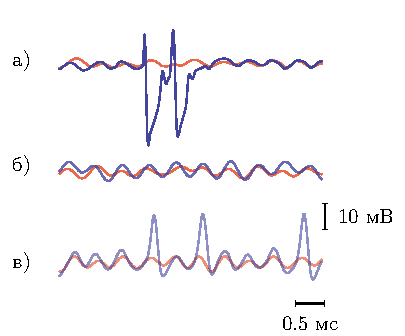
\includegraphics[]{img/img_1a}
				\caption[]{Различные виды колебаний в нейронах ствола головного мозга \cite{linas}}
			\end{figure}
		\end{column}
		\begin{column}{0.49\textwidth}
			\begin{figure}[h]
				\centering

				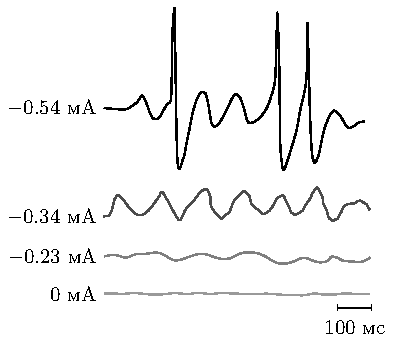
\includegraphics[]{img/img_1d}	
				\caption[]{Зависимость динамики колебаний в нейронах коры головного мозга от тока стимуляции\cite{linas}}
			\end{figure}
		\end{column}
	\end{columns}
\end{frame}
%%%%%%%%%%%%%%%%%%%%%%%%%%%%%%%%%%%%%%%%%%%%%%%%%%%%%%%%%%%%%
\subsection{Генератор Ван-дер-Поля: фазовый портрет}
\begin{frame}[t]
	\frametitle{Генератор Ван-дер-Поля: фазовый портрет}
	\vspace{-1.2em}
	% \vspace{1em}
		
	\begin{columns}
		\begin{column}{0.49\textwidth}
			\begin{figure}[h]
				\centering
				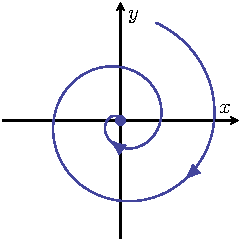
\includegraphics[scale=0.99]{img/img_2a}
				\caption{$\gamma<0$:\\ устойчивый фокус}
			\end{figure}
		\end{column}
		\begin{column}{0.49\textwidth}
			\begin{figure}[h]
				\centering
				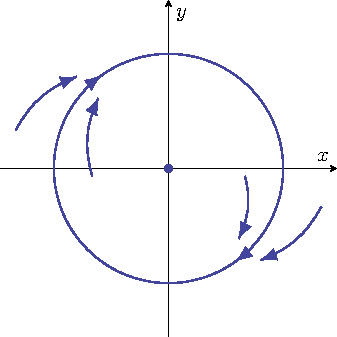
\includegraphics[scale=0.99]{img/img_2b}
				\caption{$\gamma>0$:\\ предельный цикл}
			\end{figure}
		\end{column}
	\end{columns}	
	\vspace{0.5em}
	\begin{columns}[c]
		% \begin{column}{0.49\textwidth}
		% \centering
		% В данной системе реализуются подпороговые колебания:
		% % При $\gamma=0$ происходит бифуркация Андронова-Хопфа и рождается предельный цикл
		% \end{column}
		\begin{column}{0.99\textwidth}
	\begin{equation*}
		\left\{
		\begin{aligned}
			\diff{y}{t} & =\mu(\gamma-x^2)y-\omega^2x\\%; \qquad
			\diff{x}{t}  &=y, \quad \mu \ll 1
		\end{aligned}
		\right.
	\end{equation*}		
		\end{column}
	\end{columns}
\end{frame}
%%%%%%%%%%%%%%%%%%%%%%%%%%%%%%%%%%%%%%%%%%%%%%%%%%%%%%%%%%%%%
\subsection{Модель ФитцХью-Нагумо: фазовый портрет}
\begin{frame}[t]
	\frametitle{Модель ФитцХью-Нагумо: фазовый портрет}
	% Способность к генерации спайков реализуется с помощью модели ФХН. Это простейшая система, обладающая порогом возбуждения:
	% \vspace{1em}
	\begin{columns}[c]	
		\begin{column}{0.59\textwidth}
			\vspace{-2em}
			\begin{figure}[h]
				\centering
				\hspace{1em}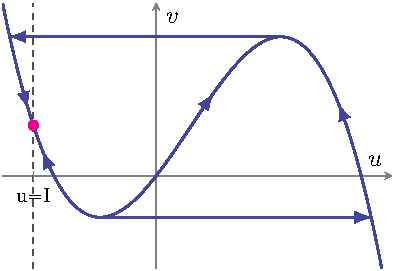
\includegraphics[]{img/img_3a}
				% \caption{3-уровневая среда}
			\end{figure}
			\vspace{-2em}
			\begin{figure}[h]
				\centering
				\hspace{1em}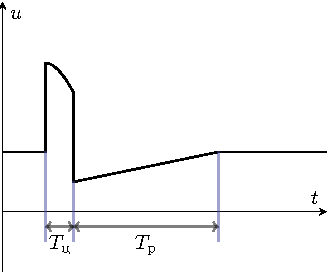
\includegraphics[]{img/img_3b}
				% \caption{3-уровневая среда}
			\end{figure}
		\end{column}
		\begin{column}{0.39\textwidth}
			$
				\left\{
				\begin{aligned}
					\diff{u}{t} & =f(u)-v           \\
					\diff{v}{t} & =\varepsilon(u-I)
				\end{aligned}
				\right.
			$\\
			\vspace{1em}
			$I$ -- параметр порога возбуждения\\
			\vspace{1em}
			$f(u)$ -- кубическая функция\\
			\vspace{1em}
			$\varepsilon \ll 1$ -- малый параметр
		\end{column}
	\end{columns}
\end{frame}
%%%%%%%%%%%%%%%%%%%%%%%%%%%%%%%%%%%%%%%%%%%%%%%%%%%%%%%%%%%%%
\subsection{Компьютерная модель Некоркина}
\begin{frame}%[bg]
	\frametitle{Математическая модель нейрона}

		% \vspace{-1em}
	
	\begin{columns}[b]
		\begin{column}{0.60\textwidth}
			% \vspace{-3em}
			\begin{equation*}
				\left\{
				\begin{aligned}
					\varepsilon_1\diff{u}{t} & =f(u)-v-d\cdot x\\
					\diff{v}{t} & =\varepsilon_2(u-I)\\
					\diff{x}{t} & =y\\
					\diff{y}{t} & =\mu(\Gamma(u,I)-x^2)y-\omega^2\cdot x
				\end{aligned}
				\right.
			\end{equation*}
		\end{column}
		\begin{column}{0.40\textwidth}
			$f(u)=u(1-u)(u-a)$\\
			\vspace{0.7em}
			$\Gamma(u,I)=\gamma(1-\alpha I +\beta u)$\\
			\vspace{0.7em}
			\begin{columns}[t]
			\begin{column}{0.49\textwidth}
				$a=0.1$\\
				$\varepsilon_1=0.001$\\
				$\varepsilon_2=1.5$\\
				$\gamma=0.21$\\
				$\omega=1$\\
			\end{column}
			\begin{column}{0.49\textwidth}
				$\alpha=5$\\
				$\beta=10$\\
				$I=-0.09$\\
				$d=0.85$\\
			\end{column}			
			\end{columns}
		\end{column}
	\end{columns}
	\begin{figure}[h]
		% \hspace{-2em}
		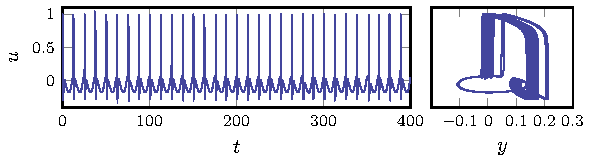
\includegraphics[scale=1]{img/limit}
		% \caption{}
	\end{figure}
\end{frame}
%%%%%%%%%%%%%%%%%%%%%%%%%%%%%%%%%%%%%%%%%%%%%%%%%%%%%%%%%%%%%
\subsection{Характерные режимы модели}
\begin{frame}%[bg]
	\frametitle{Характерные режимы модели}
		% \vspace{-2em}
	\begin{figure}[h]
		\hspace{0em}
		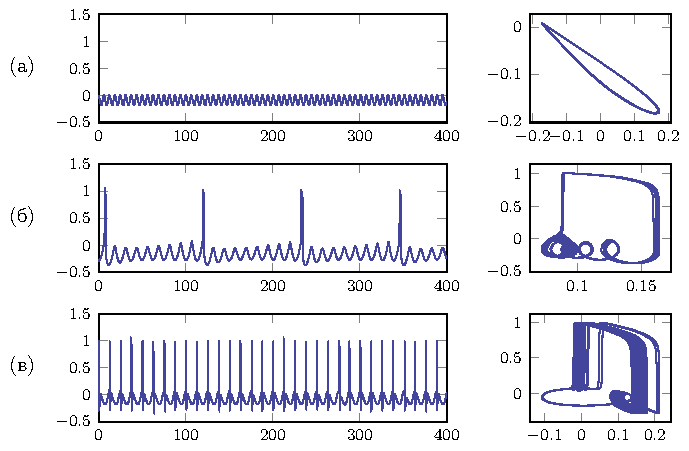
\includegraphics[scale=1]{img/img_4}
		% \caption{}
	\end{figure}
	
	% \begin{columns}[t]
	% 	\begin{column}{0.60\textwidth}
	% 		\vspace{-3em}
	% 		\begin{equation*}
	% 			\left\{
	% 			\begin{aligned}
	% 				\varepsilon_1\diff{u}{t} & =f(u)-v-d\cdot x\\
	% 				\diff{v}{t} & =\varepsilon_2(u-I)\\
	% 				\diff{x}{t} & =y\\
	% 				\diff{y}{t} & =\mu(\Gamma(u,I)-x^2)y-\Omega^2(u,I)\cdot x
	% 			\end{aligned}
	% 			\right.
	% 		\end{equation*}
	% 	\end{column}
	% 	\begin{column}{0.2\textwidth}
	% 		$a=0.1$\\
	% 		$\varepsilon_1=0.001$\\
	% 		$\varepsilon_2=1.5$\\
	% 		$\gamma=0.21$\\
	% 		$\omega=1$\\
	% 	\end{column}
	% 	\begin{column}{0.19\textwidth}
	% 		$\alpha=5$\\
	% 		$\beta=10$\\
	% 		$I=-0.09$\\
	% 		$d=0.85$\\
	% 	\end{column}		
	% \end{columns}
\end{frame}
%%%%%%%%%%%%%%%%%%%%%%%%%%%%%%%%%%%%%%%%%%%%%%%%%%%%%%%%%%%%%
\subsection{Схема экспериментальной установки}
\begin{frame}[t]%[bg]
	\frametitle{Схема экспериментальной установки}
	\vspace{-1em}
	\begin{figure}[h]
		% \hspace{-2em}
		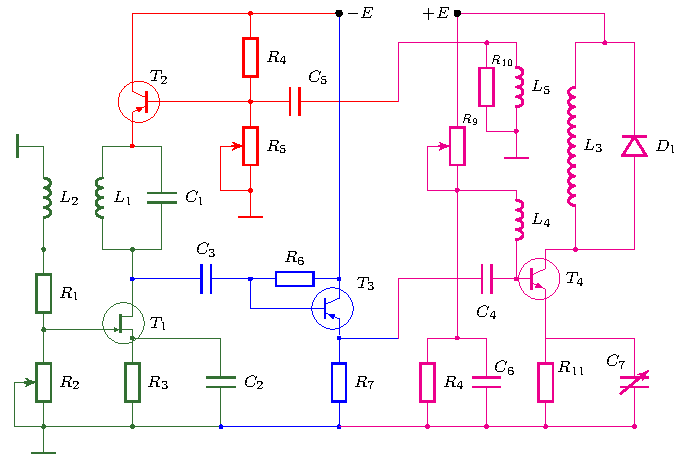
\includegraphics[width=0.86\linewidth]{img/img_6}
		% \caption{}
	\end{figure}
	\vspace{-0.5em}
	\begin{columns}
		\begin{column}{0.49\textwidth}%\centering
			\sq{black!90} -- генератор Ван-дер-Поля\\
			\sq{red} -- эмиттерный повторитель
		\end{column}
		\begin{column}{0.49\textwidth}%\centering
			\sq{blue} -- эмиттерный повторитель\\
			\sq{lightgreen} -- блокинг-генератор
		\end{column}
	\end{columns}		
\end{frame}
%%%%%%%%%%%%%%%%%%%%%%%%%%%%%%%%%%%%%%%%%%%%%%%%%%%%%%%%%%%%%
\section{Результаты эксперимента}
\subsection{Подпороговые колебания}
\begin{frame}%[bg]
	\frametitle{Подпороговые колебания}
	\begin{figure}[h]
		\hspace{-2em}
		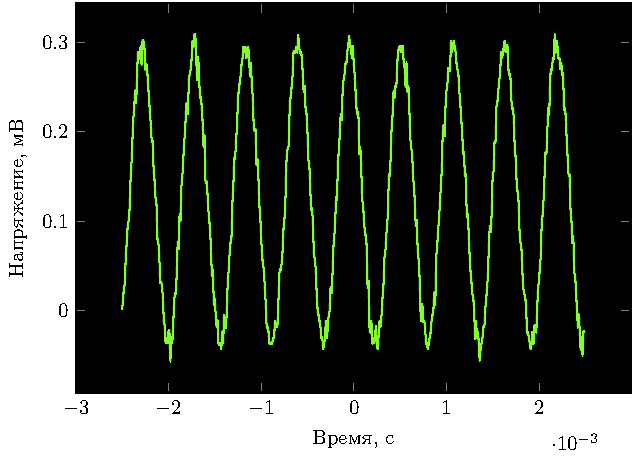
\includegraphics[]{img/osci}
		% \caption{}
	\end{figure}
\end{frame}
%%%%%%%%%%%%%%%%%%%%%%%%%%%%%%%%%%%%%%%%%%%%%%%%%%%%%%%%%%%%%
\subsection{Один спайк на несколько периодов}
\begin{frame}%[bg]
	\frametitle{Один спайк на несколько периодов}
	\begin{figure}[h]
		\hspace{-2em}
		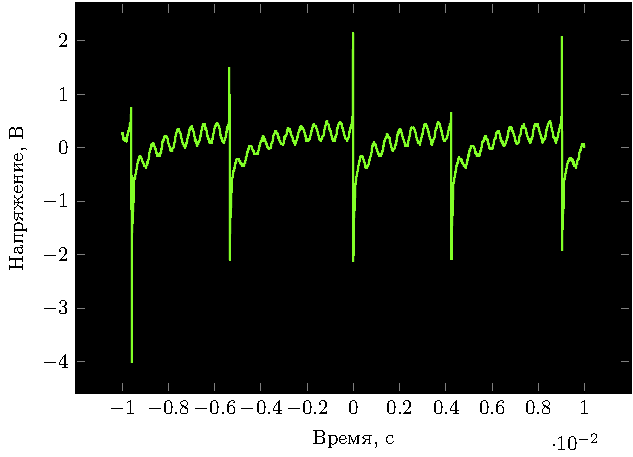
\includegraphics[]{img/spike}
		% \caption{}
	\end{figure}
\end{frame}
%%%%%%%%%%%%%%%%%%%%%%%%%%%%%%%%%%%%%%%%%%%%%%%%%%%%%%%%%%%%%
\subsection{Один спайк на период}
\begin{frame}%[bg]
	\frametitle{Один спайк на период}
	\begin{figure}[h]
		\hspace{-2em}
		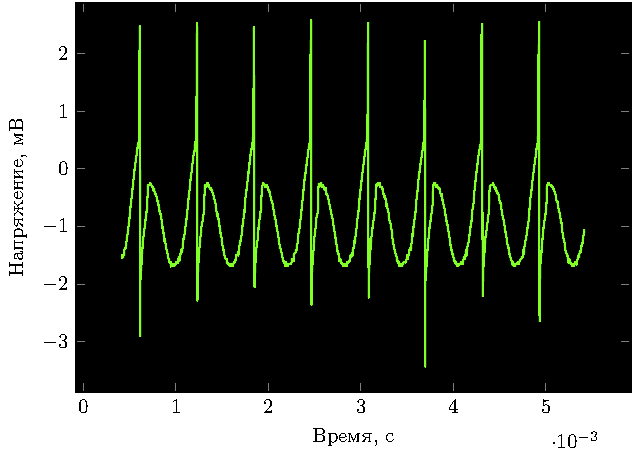
\includegraphics[]{img/onespike}
		% \caption{}
	\end{figure}
\end{frame}
%%%%%%%%%%%%%%%%%%%%%%%%%%%%%%%%%%%%%%%%%%%%%%%%%%%%%%%%%%%%%
\subsection{Два спайка на периоде}
\begin{frame}%[bg]
	\frametitle{Два спайка на периоде}
	\begin{figure}[h]
		\hspace{-2em}
		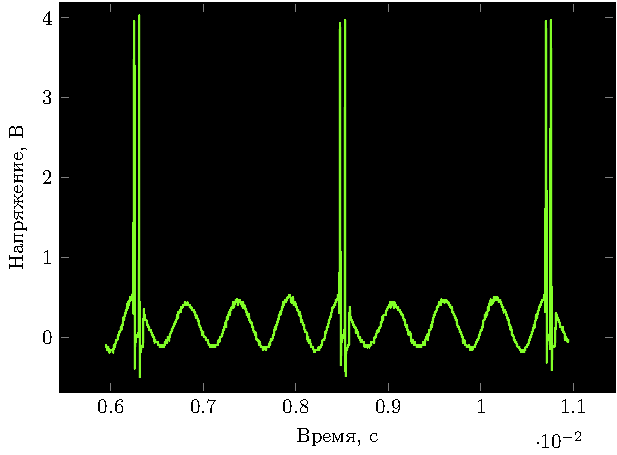
\includegraphics[]{img/twospike}
		% \caption{}
	\end{figure}
\end{frame}
%%%%%%%%%%%%%%%%%%%%%%%%%%%%%%%%%%%%%%%%%%%%%%%%%%%%%%%%%%%%%
\subsection{Спайк-берст}
\begin{frame}%[bg]
	\frametitle{Спайк-берст}
	\begin{figure}[h]
		% \hspace{-1.3em}
		% \centering
		\hspace{-2em}
		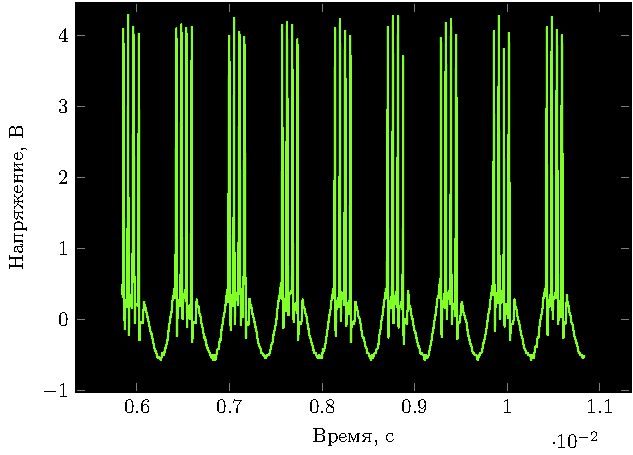
\includegraphics[]{img/berst}
		% \vspace{-1.5em}
		% \caption{Эксперимент}
	\end{figure}
	% \begin{figure}[h]
	% % \vspace{-1em}
	% 	% \hspace{-2em}
	% 	\centering
	% 	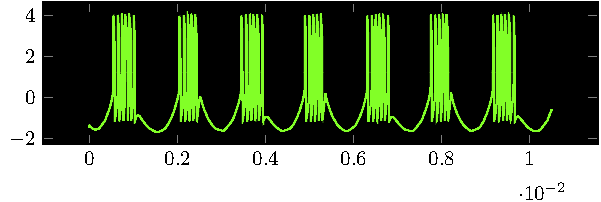
\includegraphics[]{img/berst_matlab}
	% 	% \vspace{-1.5em}
	% 	\caption{Компьютерная модель}
	% \end{figure}	
\end{frame}
%%%%%%%%%%%%%%%%%%%%%%%%%%%%%%%%%%%%%%%%%%%%%%%%%%%%%%%%%%%%%
\subsection{Влияние потенциала запирания $b_0$}
\begin{frame}%[bg]
	\frametitle{Влияние потенциала запирания $b_0$}
	\begin{figure}[h]
		% \hspace{2em}
		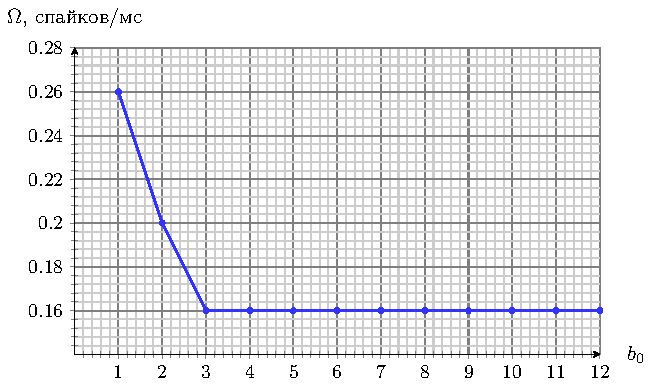
\includegraphics[]{img/b0}
		\caption{Зависимость частоты спайков от величины \\потенциала запирания $b_0$ }
	\end{figure}
\end{frame}
%%%%%%%%%%%%%%%%%%%%%%%%%%%%%%%%%%%%%%%%%%%%%%%%%%%%%%%%%%%%%
\subsection{Влияние времени релаксации на частоту спайков}
\begin{frame}%[bg]
	\frametitle{Влияние времени релаксации на частоту спайков}
	\begin{figure}[h]
		% \hspace{2em}
		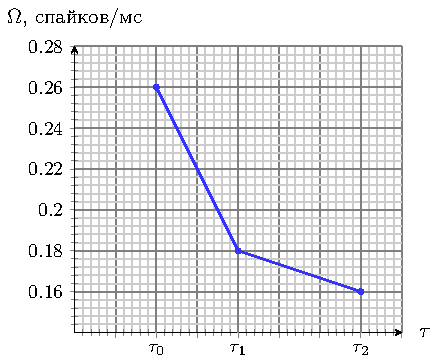
\includegraphics[]{img/ntau2}
		\caption{Зависимость частоты спайков от времени релаксации $\tau \sim C$ -- емкости конденсатора в цепи блокинг-генератора}  
	\end{figure} 
\end{frame}

%%%%%%%%%%%%%%%%%%%%%%%%%%%%%%%%%%%%%%%%%%%%%%%%%%%%%%%%%%%%%
\section{Заключение}
\subsection{Выводы}
\begin{frame}
	\frametitle{Выводы}
	\begin{enumerate}
		\item Осуществлено знакомство с моделью нейрона с подпороговыми колебаниями
		\item Качественно исследованы уравнения, соответствующие квазигармоническим колебаниям и порогу возбуждения
		\item Получены подпороговые колебания, спайк и спайк-берст режим на экспериментальной установке
		\item Реализована компьютерная модель системы, на которой был получен спайк-берст режим, показано качественное соответствие режиму, полученному эксперементально
	\end{enumerate}
\end{frame}
%%%%%%%%%%%%%%%%%%%%%%%%%%%%%%%%%%%%%%%%%%%%%%%%%%%%%%%%%%
\begin{frame}[plain]
	\frametitle{Список литературы}
	\setbeamertemplate{bibliography item}[text]
	\setbeamercolor{bibliography item}{fg=black}
	\setbeamercolor{bibliography entry title}{fg=black}
	\setbeamercolor{bibliography entry author}{fg=black}
	\setbeamercolor{bibliography entry journal}{fg=black}
	\setbeamercolor{bibliography entry note}{fg=black}
	\begin{thebibliography}{3}
	\bibitem{linas}
		R.Linas ,R.Yarom. Oscillatory properties of guinea-pig inferior olivary neurones and their pharmacological modulation: an \textit{in vitro} study. ---J.Physiol, 1986, т. 376, 163 с.
	\bibitem{andronov}
		Андронов А.А., Витт А.А., Хайкин С.Э. Теория колебаний. --- М.:ФизМатИзд, 1959, 916 с.
	\bibitem{hod}
		Ходжкин А. Нервный импульс. --- М.:Мир, 1965, 126 с.
	\end{thebibliography}
\end{frame}
\subsection{Спасибо за внимание}
\begin{frame}[plain]
	\vspace{4cm}
	\begin{center}
		\Huge
		Спасибо за внимание!
	\end{center}
	\vspace{2.5cm}
	\begin{center}
		\color{black!60!white}
		Презентация подготовлена в издательской \\
		системе LaTeX с использованием пакетов \\
		PGF/TikZ и Beamer
	\end{center}
\end{frame}
\end{document}